\documentclass[twoside]{book}

% Packages required by doxygen
\usepackage{fixltx2e}
\usepackage{calc}
\usepackage{doxygen}
\usepackage[export]{adjustbox} % also loads graphicx
\usepackage{graphicx}
\usepackage[utf8]{inputenc}
\usepackage{makeidx}
\usepackage{multicol}
\usepackage{multirow}
\PassOptionsToPackage{warn}{textcomp}
\usepackage{textcomp}
\usepackage[nointegrals]{wasysym}
\usepackage[table]{xcolor}

% Font selection
\usepackage[T1]{fontenc}
\usepackage[scaled=.90]{helvet}
\usepackage{courier}
\usepackage{amssymb}
\usepackage{sectsty}
\renewcommand{\familydefault}{\sfdefault}
\allsectionsfont{%
  \fontseries{bc}\selectfont%
  \color{darkgray}%
}
\renewcommand{\DoxyLabelFont}{%
  \fontseries{bc}\selectfont%
  \color{darkgray}%
}
\newcommand{\+}{\discretionary{\mbox{\scriptsize$\hookleftarrow$}}{}{}}

% Page & text layout
\usepackage{geometry}
\geometry{%
  a4paper,%
  top=2.5cm,%
  bottom=2.5cm,%
  left=2.5cm,%
  right=2.5cm%
}
\tolerance=750
\hfuzz=15pt
\hbadness=750
\setlength{\emergencystretch}{15pt}
\setlength{\parindent}{0cm}
\setlength{\parskip}{3ex plus 2ex minus 2ex}
\makeatletter
\renewcommand{\paragraph}{%
  \@startsection{paragraph}{4}{0ex}{-1.0ex}{1.0ex}{%
    \normalfont\normalsize\bfseries\SS@parafont%
  }%
}
\renewcommand{\subparagraph}{%
  \@startsection{subparagraph}{5}{0ex}{-1.0ex}{1.0ex}{%
    \normalfont\normalsize\bfseries\SS@subparafont%
  }%
}
\makeatother

% Headers & footers
\usepackage{fancyhdr}
\pagestyle{fancyplain}
\fancyhead[LE]{\fancyplain{}{\bfseries\thepage}}
\fancyhead[CE]{\fancyplain{}{}}
\fancyhead[RE]{\fancyplain{}{\bfseries\leftmark}}
\fancyhead[LO]{\fancyplain{}{\bfseries\rightmark}}
\fancyhead[CO]{\fancyplain{}{}}
\fancyhead[RO]{\fancyplain{}{\bfseries\thepage}}
\fancyfoot[LE]{\fancyplain{}{}}
\fancyfoot[CE]{\fancyplain{}{}}
\fancyfoot[RE]{\fancyplain{}{\bfseries\scriptsize Generated by Doxygen }}
\fancyfoot[LO]{\fancyplain{}{\bfseries\scriptsize Generated by Doxygen }}
\fancyfoot[CO]{\fancyplain{}{}}
\fancyfoot[RO]{\fancyplain{}{}}
\renewcommand{\footrulewidth}{0.4pt}
\renewcommand{\chaptermark}[1]{%
  \markboth{#1}{}%
}
\renewcommand{\sectionmark}[1]{%
  \markright{\thesection\ #1}%
}

% Indices & bibliography
\usepackage{natbib}
\usepackage[titles]{tocloft}
\setcounter{tocdepth}{3}
\setcounter{secnumdepth}{5}
\makeindex

% Hyperlinks (required, but should be loaded last)
\usepackage{ifpdf}
\ifpdf
  \usepackage[pdftex,pagebackref=true]{hyperref}
\else
  \usepackage[ps2pdf,pagebackref=true]{hyperref}
\fi
\hypersetup{%
  colorlinks=true,%
  linkcolor=blue,%
  citecolor=blue,%
  unicode%
}

% Custom commands
\newcommand{\clearemptydoublepage}{%
  \newpage{\pagestyle{empty}\cleardoublepage}%
}

\usepackage{caption}
\captionsetup{labelsep=space,justification=centering,font={bf},singlelinecheck=off,skip=4pt,position=top}

%===== C O N T E N T S =====

\begin{document}

% Titlepage & ToC
\hypersetup{pageanchor=false,
             bookmarksnumbered=true,
             pdfencoding=unicode
            }
\pagenumbering{alph}
\begin{titlepage}
\vspace*{7cm}
\begin{center}%
{\Large My Project }\\
\vspace*{1cm}
{\large Generated by Doxygen 1.8.14}\\
\end{center}
\end{titlepage}
\clearemptydoublepage
\pagenumbering{roman}
\tableofcontents
\clearemptydoublepage
\pagenumbering{arabic}
\hypersetup{pageanchor=true}

%--- Begin generated contents ---
\chapter{Namespace Index}
\section{Namespace List}
Here is a list of all documented namespaces with brief descriptions\+:\begin{DoxyCompactList}
\item\contentsline{section}{\hyperlink{namespacemessengerbot_1_1views}{messengerbot.\+views} }{\pageref{namespacemessengerbot_1_1views}}{}
\end{DoxyCompactList}

\chapter{Hierarchical Index}
\section{Class Hierarchy}
This inheritance list is sorted roughly, but not completely, alphabetically\+:\begin{DoxyCompactList}
\item Model\begin{DoxyCompactList}
\item \contentsline{section}{messengerbot.\+models.\+address}{\pageref{classmessengerbot_1_1models_1_1address}}{}
\item \contentsline{section}{messengerbot.\+models.\+country}{\pageref{classmessengerbot_1_1models_1_1country}}{}
\item \contentsline{section}{messengerbot.\+models.\+language}{\pageref{classmessengerbot_1_1models_1_1language}}{}
\item \contentsline{section}{messengerbot.\+models.\+mode\+\_\+of\+\_\+contact}{\pageref{classmessengerbot_1_1models_1_1mode__of__contact}}{}
\item \contentsline{section}{messengerbot.\+models.\+order}{\pageref{classmessengerbot_1_1models_1_1order}}{}
\item \contentsline{section}{messengerbot.\+models.\+place}{\pageref{classmessengerbot_1_1models_1_1place}}{}
\item \contentsline{section}{messengerbot.\+models.\+status}{\pageref{classmessengerbot_1_1models_1_1status}}{}
\item \contentsline{section}{messengerbot.\+models.\+status\+\_\+code}{\pageref{classmessengerbot_1_1models_1_1status__code}}{}
\item \contentsline{section}{messengerbot.\+models.\+type\+\_\+of\+\_\+box}{\pageref{classmessengerbot_1_1models_1_1type__of__box}}{}
\item \contentsline{section}{messengerbot.\+models.\+type\+\_\+of\+\_\+collection}{\pageref{classmessengerbot_1_1models_1_1type__of__collection}}{}
\item \contentsline{section}{messengerbot.\+models.\+type\+\_\+of\+\_\+service}{\pageref{classmessengerbot_1_1models_1_1type__of__service}}{}
\item \contentsline{section}{messengerbot.\+models.\+type\+\_\+of\+\_\+shipment}{\pageref{classmessengerbot_1_1models_1_1type__of__shipment}}{}
\item \contentsline{section}{messengerbot.\+models.\+user}{\pageref{classmessengerbot_1_1models_1_1user}}{}
\end{DoxyCompactList}
\item View\begin{DoxyCompactList}
\item \contentsline{section}{messengerbot.\+views.\+My\+Chat\+Bot\+View}{\pageref{classmessengerbot_1_1views_1_1MyChatBotView}}{}
\end{DoxyCompactList}
\item Test\+Case\begin{DoxyCompactList}
\item \contentsline{section}{messengerbot.\+tests.\+Test\+Verify\+Token}{\pageref{classmessengerbot_1_1tests_1_1TestVerifyToken}}{}
\end{DoxyCompactList}
\end{DoxyCompactList}

\chapter{Class Index}
\section{Class List}
Here are the classes, structs, unions and interfaces with brief descriptions\+:\begin{DoxyCompactList}
\item\contentsline{section}{\hyperlink{classmessengerbot_1_1models_1_1address}{messengerbot.\+models.\+address} }{\pageref{classmessengerbot_1_1models_1_1address}}{}
\item\contentsline{section}{\hyperlink{classmessengerbot_1_1models_1_1country}{messengerbot.\+models.\+country} }{\pageref{classmessengerbot_1_1models_1_1country}}{}
\item\contentsline{section}{\hyperlink{classmessengerbot_1_1models_1_1language}{messengerbot.\+models.\+language} }{\pageref{classmessengerbot_1_1models_1_1language}}{}
\item\contentsline{section}{\hyperlink{classmessengerbot_1_1models_1_1mode__of__contact}{messengerbot.\+models.\+mode\+\_\+of\+\_\+contact} }{\pageref{classmessengerbot_1_1models_1_1mode__of__contact}}{}
\item\contentsline{section}{\hyperlink{classmessengerbot_1_1views_1_1MyChatBotView}{messengerbot.\+views.\+My\+Chat\+Bot\+View} }{\pageref{classmessengerbot_1_1views_1_1MyChatBotView}}{}
\item\contentsline{section}{\hyperlink{classmessengerbot_1_1models_1_1order}{messengerbot.\+models.\+order} }{\pageref{classmessengerbot_1_1models_1_1order}}{}
\item\contentsline{section}{\hyperlink{classmessengerbot_1_1models_1_1place}{messengerbot.\+models.\+place} }{\pageref{classmessengerbot_1_1models_1_1place}}{}
\item\contentsline{section}{\hyperlink{classmessengerbot_1_1models_1_1status}{messengerbot.\+models.\+status} }{\pageref{classmessengerbot_1_1models_1_1status}}{}
\item\contentsline{section}{\hyperlink{classmessengerbot_1_1models_1_1status__code}{messengerbot.\+models.\+status\+\_\+code} }{\pageref{classmessengerbot_1_1models_1_1status__code}}{}
\item\contentsline{section}{\hyperlink{classmessengerbot_1_1tests_1_1TestVerifyToken}{messengerbot.\+tests.\+Test\+Verify\+Token} }{\pageref{classmessengerbot_1_1tests_1_1TestVerifyToken}}{}
\item\contentsline{section}{\hyperlink{classmessengerbot_1_1models_1_1type__of__box}{messengerbot.\+models.\+type\+\_\+of\+\_\+box} }{\pageref{classmessengerbot_1_1models_1_1type__of__box}}{}
\item\contentsline{section}{\hyperlink{classmessengerbot_1_1models_1_1type__of__collection}{messengerbot.\+models.\+type\+\_\+of\+\_\+collection} }{\pageref{classmessengerbot_1_1models_1_1type__of__collection}}{}
\item\contentsline{section}{\hyperlink{classmessengerbot_1_1models_1_1type__of__service}{messengerbot.\+models.\+type\+\_\+of\+\_\+service} }{\pageref{classmessengerbot_1_1models_1_1type__of__service}}{}
\item\contentsline{section}{\hyperlink{classmessengerbot_1_1models_1_1type__of__shipment}{messengerbot.\+models.\+type\+\_\+of\+\_\+shipment} }{\pageref{classmessengerbot_1_1models_1_1type__of__shipment}}{}
\item\contentsline{section}{\hyperlink{classmessengerbot_1_1models_1_1user}{messengerbot.\+models.\+user} }{\pageref{classmessengerbot_1_1models_1_1user}}{}
\end{DoxyCompactList}

\chapter{Namespace Documentation}
\hypertarget{namespacemessengerbot_1_1views}{}\section{messengerbot.\+views Namespace Reference}
\label{namespacemessengerbot_1_1views}\index{messengerbot.\+views@{messengerbot.\+views}}
\subsection*{Classes}
\begin{DoxyCompactItemize}
\item 
class \hyperlink{classmessengerbot_1_1views_1_1MyChatBotView}{My\+Chat\+Bot\+View}
\end{DoxyCompactItemize}
\subsection*{Functions}
\begin{DoxyCompactItemize}
\item 
\mbox{\Hypertarget{namespacemessengerbot_1_1views_ab1f6e22eebdb8099aa11080d19d6d998}\label{namespacemessengerbot_1_1views_ab1f6e22eebdb8099aa11080d19d6d998}} 
def {\bfseries user\+\_\+details} (fbid)
\item 
\mbox{\Hypertarget{namespacemessengerbot_1_1views_a197d2929ea4b8b6832965a1d66b60fd6}\label{namespacemessengerbot_1_1views_a197d2929ea4b8b6832965a1d66b60fd6}} 
def {\bfseries api\+\_\+ai\+\_\+webhook} (request)
\item 
def \hyperlink{namespacemessengerbot_1_1views_a1640e1dc00146c9ca843d7a746cf122d}{post\+\_\+facebook\+\_\+message} (fbid, message\+\_\+text)
\item 
\mbox{\Hypertarget{namespacemessengerbot_1_1views_ad89592c43fcbe0c4cb07945221e109fc}\label{namespacemessengerbot_1_1views_ad89592c43fcbe0c4cb07945221e109fc}} 
def {\bfseries index} (request)
\item 
\mbox{\Hypertarget{namespacemessengerbot_1_1views_acb353edab49a475685bc8c8830e1d91e}\label{namespacemessengerbot_1_1views_acb353edab49a475685bc8c8830e1d91e}} 
def {\bfseries otp\+\_\+form} (request)
\item 
\mbox{\Hypertarget{namespacemessengerbot_1_1views_a690221e7f4637eb42ba9d734fb2f2493}\label{namespacemessengerbot_1_1views_a690221e7f4637eb42ba9d734fb2f2493}} 
def {\bfseries receipt} (request)
\item 
\mbox{\Hypertarget{namespacemessengerbot_1_1views_acc602ca40d1ea9e8630f8af91fed19c9}\label{namespacemessengerbot_1_1views_acc602ca40d1ea9e8630f8af91fed19c9}} 
def {\bfseries track} (request)
\item 
def \hyperlink{namespacemessengerbot_1_1views_a0422c7b7111b5e4de6bc606e67c554ef}{identity\+\_\+confirm} (request)
\item 
\mbox{\Hypertarget{namespacemessengerbot_1_1views_a56c122fb7a1524b4722761a9d0093554}\label{namespacemessengerbot_1_1views_a56c122fb7a1524b4722761a9d0093554}} 
def {\bfseries help} (request)
\item 
def \hyperlink{namespacemessengerbot_1_1views_a001bef22e3a7e6c9385e486f6e22b679}{greeting\+\_\+text} ()
\item 
\mbox{\Hypertarget{namespacemessengerbot_1_1views_ac320ab20a7fa639fb9ba9207e5ab7942}\label{namespacemessengerbot_1_1views_ac320ab20a7fa639fb9ba9207e5ab7942}} 
def {\bfseries greeting\+\_\+button} ()
\end{DoxyCompactItemize}
\subsection*{Variables}
\begin{DoxyCompactItemize}
\item 
\mbox{\Hypertarget{namespacemessengerbot_1_1views_acc5db9b1386d0938d9b1c07a9c83604e}\label{namespacemessengerbot_1_1views_acc5db9b1386d0938d9b1c07a9c83604e}} 
string {\bfseries V\+E\+R\+I\+F\+Y\+\_\+\+T\+O\+K\+EN} = \textquotesingle{}dhlchatbot\textquotesingle{}
\item 
\mbox{\Hypertarget{namespacemessengerbot_1_1views_a22c4a4c96dbae1b10bd243bdbd7b0505}\label{namespacemessengerbot_1_1views_a22c4a4c96dbae1b10bd243bdbd7b0505}} 
string {\bfseries P\+A\+G\+E\+\_\+\+A\+C\+C\+E\+S\+S\+\_\+\+T\+O\+K\+EN} = \textquotesingle{}E\+A\+A\+G\+W93s\+Ngsg\+B\+A\+Kn6\+Me\+Sm\+L\+H\+Q\+Q\+Br\+S\+Fo\+J\+Z\+Ba3\+Z\+Cp\+A\+Z\+Bi\+S\+Dx\+M\+L\+Xsh\+Nd7\+P\+K1d\+R\+S\+D\+O1\+X\+H4d\+Z\+Bnf\+Bs\+Z\+B\+Pxs\+Awh9\+B\+Nz\+H\+Ky94a\+H\+Pa\+L4\+Woqdx\+Yv\+Wovsti\+Yle\+J\+Z\+C09\+F\+Ek\+Ooen\+A\+Fo\+Wxss5\+N\+Ly\+X\+Gdc\+Pz1\+V\+I46\+Oa\+E\+W5\+Ll\+T\+Z\+Ap\+Vlnw\+Fzf\+F3n\+Gl1w\+W5tg\+Z\+D\+ZD\textquotesingle{}
\end{DoxyCompactItemize}


\subsection{Detailed Description}
\begin{DoxyVerb}Documentation for this module:
This module of django handles all the requets from the Facebook bot and works via a webhook to get an instant update of a message recieved and replies instantly by parsing specific conditions mentioned in this module for appropriate reply. 
\end{DoxyVerb}
 

\subsection{Function Documentation}
\mbox{\Hypertarget{namespacemessengerbot_1_1views_a001bef22e3a7e6c9385e486f6e22b679}\label{namespacemessengerbot_1_1views_a001bef22e3a7e6c9385e486f6e22b679}} 
\index{messengerbot\+::views@{messengerbot\+::views}!greeting\+\_\+text@{greeting\+\_\+text}}
\index{greeting\+\_\+text@{greeting\+\_\+text}!messengerbot\+::views@{messengerbot\+::views}}
\subsubsection{\texorpdfstring{greeting\+\_\+text()}{greeting\_text()}}
{\footnotesize\ttfamily def messengerbot.\+views.\+greeting\+\_\+text (\begin{DoxyParamCaption}{ }\end{DoxyParamCaption})}

\begin{DoxyVerb}This function acts as a starting button when someone tries the bot for this first time .
\end{DoxyVerb}
 \mbox{\Hypertarget{namespacemessengerbot_1_1views_a0422c7b7111b5e4de6bc606e67c554ef}\label{namespacemessengerbot_1_1views_a0422c7b7111b5e4de6bc606e67c554ef}} 
\index{messengerbot\+::views@{messengerbot\+::views}!identity\+\_\+confirm@{identity\+\_\+confirm}}
\index{identity\+\_\+confirm@{identity\+\_\+confirm}!messengerbot\+::views@{messengerbot\+::views}}
\subsubsection{\texorpdfstring{identity\+\_\+confirm()}{identity\_confirm()}}
{\footnotesize\ttfamily def messengerbot.\+views.\+identity\+\_\+confirm (\begin{DoxyParamCaption}\item[{}]{request }\end{DoxyParamCaption})}

\begin{DoxyVerb}This function gets a request from javascript sdk of /otp_form(whitelisted domain for identity confirmation) to check for authenticity of the user .  
\end{DoxyVerb}
 \mbox{\Hypertarget{namespacemessengerbot_1_1views_a1640e1dc00146c9ca843d7a746cf122d}\label{namespacemessengerbot_1_1views_a1640e1dc00146c9ca843d7a746cf122d}} 
\index{messengerbot\+::views@{messengerbot\+::views}!post\+\_\+facebook\+\_\+message@{post\+\_\+facebook\+\_\+message}}
\index{post\+\_\+facebook\+\_\+message@{post\+\_\+facebook\+\_\+message}!messengerbot\+::views@{messengerbot\+::views}}
\subsubsection{\texorpdfstring{post\+\_\+facebook\+\_\+message()}{post\_facebook\_message()}}
{\footnotesize\ttfamily def messengerbot.\+views.\+post\+\_\+facebook\+\_\+message (\begin{DoxyParamCaption}\item[{}]{fbid,  }\item[{}]{message\+\_\+text }\end{DoxyParamCaption})}

\begin{DoxyVerb}Function to invoke the facebook API to send message to the dedicated user\end{DoxyVerb}
 
\chapter{Class Documentation}
\hypertarget{classmessengerbot_1_1models_1_1address}{}\section{messengerbot.\+models.\+address Class Reference}
\label{classmessengerbot_1_1models_1_1address}\index{messengerbot.\+models.\+address@{messengerbot.\+models.\+address}}
Inheritance diagram for messengerbot.\+models.\+address\+:\begin{figure}[H]
\begin{center}
\leavevmode
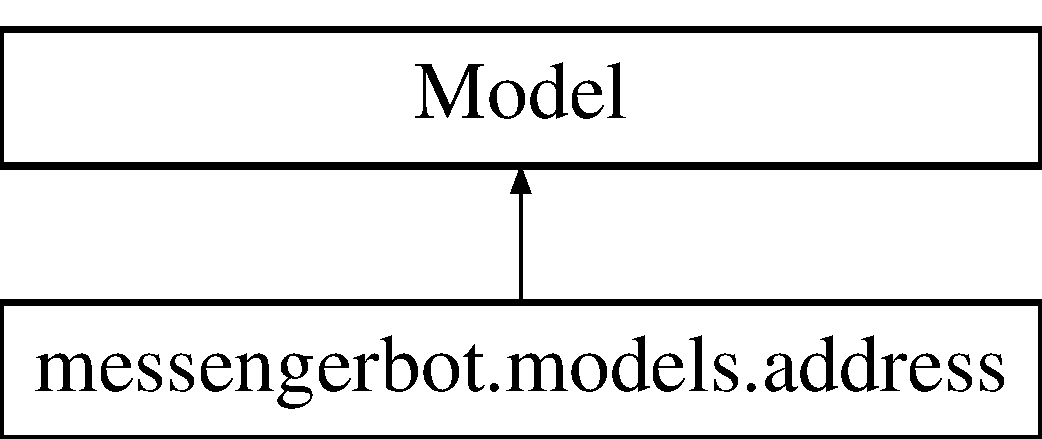
\includegraphics[height=2.000000cm]{classmessengerbot_1_1models_1_1address}
\end{center}
\end{figure}
\subsection*{Public Member Functions}
\begin{DoxyCompactItemize}
\item 
\mbox{\Hypertarget{classmessengerbot_1_1models_1_1address_a5f4ba5826fd95684762687c69473961f}\label{classmessengerbot_1_1models_1_1address_a5f4ba5826fd95684762687c69473961f}} 
def {\bfseries \+\_\+\+\_\+str\+\_\+\+\_\+} (self)
\end{DoxyCompactItemize}
\subsection*{Static Public Attributes}
\begin{DoxyCompactItemize}
\item 
\mbox{\Hypertarget{classmessengerbot_1_1models_1_1address_a85dff36c313a4437aa39e7f2a83589ed}\label{classmessengerbot_1_1models_1_1address_a85dff36c313a4437aa39e7f2a83589ed}} 
{\bfseries fbid} = models.\+Many\+To\+Many\+Field(\hyperlink{classmessengerbot_1_1models_1_1user}{user}, null = True)
\item 
\mbox{\Hypertarget{classmessengerbot_1_1models_1_1address_a549a6273b46ccb95313170df8a2f4223}\label{classmessengerbot_1_1models_1_1address_a549a6273b46ccb95313170df8a2f4223}} 
{\bfseries name} = models.\+Char\+Field(max\+\_\+length = 250 , default = \textquotesingle{}N\+U\+LL\textquotesingle{})
\item 
\mbox{\Hypertarget{classmessengerbot_1_1models_1_1address_aa4c0c585dc31e3c740efcc53e07605cc}\label{classmessengerbot_1_1models_1_1address_aa4c0c585dc31e3c740efcc53e07605cc}} 
{\bfseries address} = models.\+Char\+Field(max\+\_\+length = 250 , default = \textquotesingle{}N\+U\+LL\textquotesingle{})
\item 
\mbox{\Hypertarget{classmessengerbot_1_1models_1_1address_aebe139c4196e462074da0a624bb6219c}\label{classmessengerbot_1_1models_1_1address_aebe139c4196e462074da0a624bb6219c}} 
{\bfseries zip\+Code} = models.\+Char\+Field(max\+\_\+length = 250 , default = \textquotesingle{}N\+U\+LL\textquotesingle{})
\item 
\mbox{\Hypertarget{classmessengerbot_1_1models_1_1address_a4ebf976d2d102ed86f8df2052367ece0}\label{classmessengerbot_1_1models_1_1address_a4ebf976d2d102ed86f8df2052367ece0}} 
{\bfseries email} = models.\+Char\+Field(max\+\_\+length = 250 , default = \textquotesingle{}N\+U\+LL\textquotesingle{})
\item 
\mbox{\Hypertarget{classmessengerbot_1_1models_1_1address_a58db9d45a5fb58b321296870618deb7f}\label{classmessengerbot_1_1models_1_1address_a58db9d45a5fb58b321296870618deb7f}} 
{\bfseries phone} = models.\+Char\+Field(max\+\_\+length = 250 , default = \textquotesingle{}N\+U\+LL\textquotesingle{})
\end{DoxyCompactItemize}


The documentation for this class was generated from the following file\+:\begin{DoxyCompactItemize}
\item 
models.\+py\end{DoxyCompactItemize}

\hypertarget{classmessengerbot_1_1models_1_1country}{}\section{messengerbot.\+models.\+country Class Reference}
\label{classmessengerbot_1_1models_1_1country}\index{messengerbot.\+models.\+country@{messengerbot.\+models.\+country}}
Inheritance diagram for messengerbot.\+models.\+country\+:\begin{figure}[H]
\begin{center}
\leavevmode
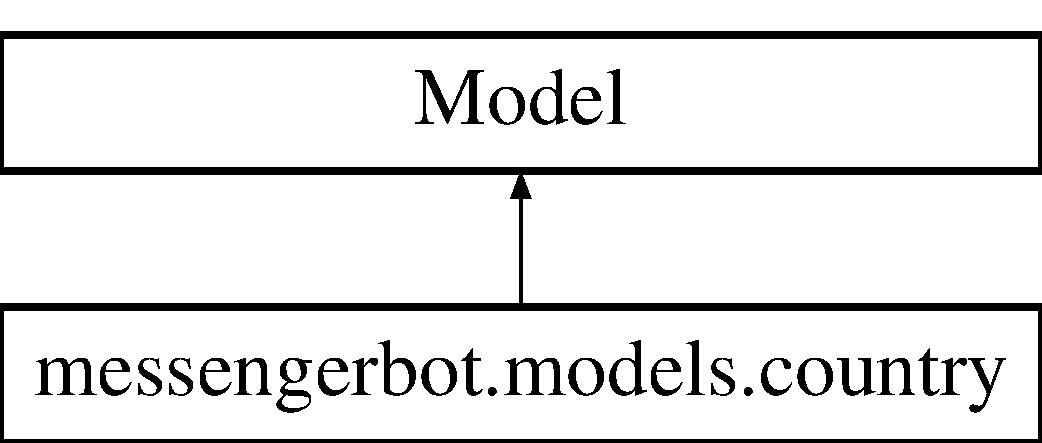
\includegraphics[height=2.000000cm]{classmessengerbot_1_1models_1_1country}
\end{center}
\end{figure}
\subsection*{Public Member Functions}
\begin{DoxyCompactItemize}
\item 
\mbox{\Hypertarget{classmessengerbot_1_1models_1_1country_a87a737d0996b7e070945370c72839e30}\label{classmessengerbot_1_1models_1_1country_a87a737d0996b7e070945370c72839e30}} 
def {\bfseries \+\_\+\+\_\+str\+\_\+\+\_\+} (self)
\end{DoxyCompactItemize}
\subsection*{Static Public Attributes}
\begin{DoxyCompactItemize}
\item 
\mbox{\Hypertarget{classmessengerbot_1_1models_1_1country_af2e57cfffa2944ef3adbd02f53146fcc}\label{classmessengerbot_1_1models_1_1country_af2e57cfffa2944ef3adbd02f53146fcc}} 
{\bfseries name} = models.\+Char\+Field(max\+\_\+length = 250 , default = \textquotesingle{}N\+U\+LL\textquotesingle{})
\end{DoxyCompactItemize}


\subsection{Detailed Description}
\begin{DoxyVerb}data of the countries DHL works in with there timezone and languages spoken\end{DoxyVerb}
\begin{DoxyVerb}countries DHL work in\end{DoxyVerb}
 

The documentation for this class was generated from the following file\+:\begin{DoxyCompactItemize}
\item 
models.\+py\end{DoxyCompactItemize}

\hypertarget{classmessengerbot_1_1models_1_1language}{}\section{messengerbot.\+models.\+language Class Reference}
\label{classmessengerbot_1_1models_1_1language}\index{messengerbot.\+models.\+language@{messengerbot.\+models.\+language}}
Inheritance diagram for messengerbot.\+models.\+language\+:\begin{figure}[H]
\begin{center}
\leavevmode
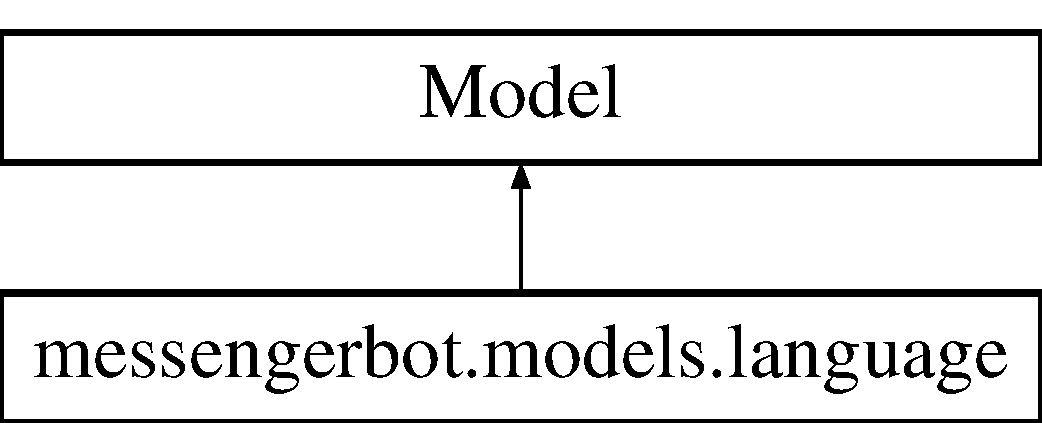
\includegraphics[height=2.000000cm]{classmessengerbot_1_1models_1_1language}
\end{center}
\end{figure}
\subsection*{Public Member Functions}
\begin{DoxyCompactItemize}
\item 
\mbox{\Hypertarget{classmessengerbot_1_1models_1_1language_a0cb14c023495e985949e8403eb4eca88}\label{classmessengerbot_1_1models_1_1language_a0cb14c023495e985949e8403eb4eca88}} 
def {\bfseries \+\_\+\+\_\+str\+\_\+\+\_\+} (self)
\end{DoxyCompactItemize}
\subsection*{Static Public Attributes}
\begin{DoxyCompactItemize}
\item 
\mbox{\Hypertarget{classmessengerbot_1_1models_1_1language_ae12a1e259f788f923b5eb031021f507d}\label{classmessengerbot_1_1models_1_1language_ae12a1e259f788f923b5eb031021f507d}} 
{\bfseries name} = models.\+Char\+Field(max\+\_\+length = 250 , default = \textquotesingle{}N\+U\+LL\textquotesingle{})
\end{DoxyCompactItemize}


\subsection{Detailed Description}
\begin{DoxyVerb}languages users of the bot speaks . \end{DoxyVerb}
 

The documentation for this class was generated from the following file\+:\begin{DoxyCompactItemize}
\item 
models.\+py\end{DoxyCompactItemize}

\hypertarget{classmessengerbot_1_1models_1_1mode__of__contact}{}\section{messengerbot.\+models.\+mode\+\_\+of\+\_\+contact Class Reference}
\label{classmessengerbot_1_1models_1_1mode__of__contact}\index{messengerbot.\+models.\+mode\+\_\+of\+\_\+contact@{messengerbot.\+models.\+mode\+\_\+of\+\_\+contact}}
Inheritance diagram for messengerbot.\+models.\+mode\+\_\+of\+\_\+contact\+:\begin{figure}[H]
\begin{center}
\leavevmode
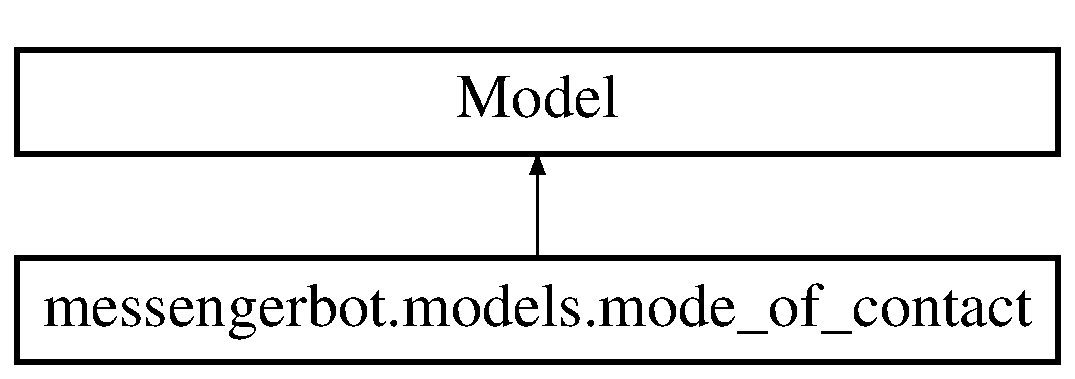
\includegraphics[height=2.000000cm]{classmessengerbot_1_1models_1_1mode__of__contact}
\end{center}
\end{figure}
\subsection*{Public Member Functions}
\begin{DoxyCompactItemize}
\item 
\mbox{\Hypertarget{classmessengerbot_1_1models_1_1mode__of__contact_a6ebd4c5bca4b5fbaa27f327d67b57b18}\label{classmessengerbot_1_1models_1_1mode__of__contact_a6ebd4c5bca4b5fbaa27f327d67b57b18}} 
def {\bfseries \+\_\+\+\_\+str\+\_\+\+\_\+} (self)
\end{DoxyCompactItemize}
\subsection*{Static Public Attributes}
\begin{DoxyCompactItemize}
\item 
\mbox{\Hypertarget{classmessengerbot_1_1models_1_1mode__of__contact_aad7efb4a0b7b09beb5faae33659984a7}\label{classmessengerbot_1_1models_1_1mode__of__contact_aad7efb4a0b7b09beb5faae33659984a7}} 
{\bfseries mode\+\_\+of\+\_\+contact} = models.\+Char\+Field(max\+\_\+length = 250 , default = \textquotesingle{}N\+U\+LL\textquotesingle{})
\end{DoxyCompactItemize}


\subsection{Detailed Description}
\begin{DoxyVerb}for mode of conact for the user like "phone " or "online\end{DoxyVerb}
 

The documentation for this class was generated from the following file\+:\begin{DoxyCompactItemize}
\item 
models.\+py\end{DoxyCompactItemize}

\hypertarget{classmessengerbot_1_1views_1_1MyChatBotView}{}\section{messengerbot.\+views.\+My\+Chat\+Bot\+View Class Reference}
\label{classmessengerbot_1_1views_1_1MyChatBotView}\index{messengerbot.\+views.\+My\+Chat\+Bot\+View@{messengerbot.\+views.\+My\+Chat\+Bot\+View}}
Inheritance diagram for messengerbot.\+views.\+My\+Chat\+Bot\+View\+:\begin{figure}[H]
\begin{center}
\leavevmode
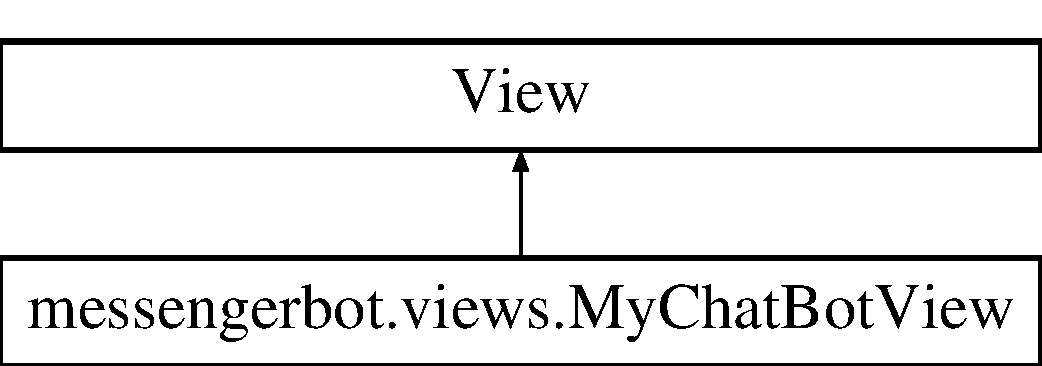
\includegraphics[height=2.000000cm]{classmessengerbot_1_1views_1_1MyChatBotView}
\end{center}
\end{figure}
\subsection*{Public Member Functions}
\begin{DoxyCompactItemize}
\item 
\mbox{\Hypertarget{classmessengerbot_1_1views_1_1MyChatBotView_a3023bcfc14b0a4a963d47ec01af604ad}\label{classmessengerbot_1_1views_1_1MyChatBotView_a3023bcfc14b0a4a963d47ec01af604ad}} 
def {\bfseries get} (self, request, args, kwargs)
\item 
\mbox{\Hypertarget{classmessengerbot_1_1views_1_1MyChatBotView_a046fb0cd8f4598904864633b1b76a0b8}\label{classmessengerbot_1_1views_1_1MyChatBotView_a046fb0cd8f4598904864633b1b76a0b8}} 
def {\bfseries dispatch} (self, request, args, kwargs)
\item 
\mbox{\Hypertarget{classmessengerbot_1_1views_1_1MyChatBotView_a60402a8e54abc2020a4ca63b84506b9a}\label{classmessengerbot_1_1views_1_1MyChatBotView_a60402a8e54abc2020a4ca63b84506b9a}} 
def {\bfseries post} (self, request, args, kwargs)
\end{DoxyCompactItemize}


The documentation for this class was generated from the following file\+:\begin{DoxyCompactItemize}
\item 
views.\+py\end{DoxyCompactItemize}

\hypertarget{classmessengerbot_1_1models_1_1order}{}\section{messengerbot.\+models.\+order Class Reference}
\label{classmessengerbot_1_1models_1_1order}\index{messengerbot.\+models.\+order@{messengerbot.\+models.\+order}}
Inheritance diagram for messengerbot.\+models.\+order\+:\begin{figure}[H]
\begin{center}
\leavevmode
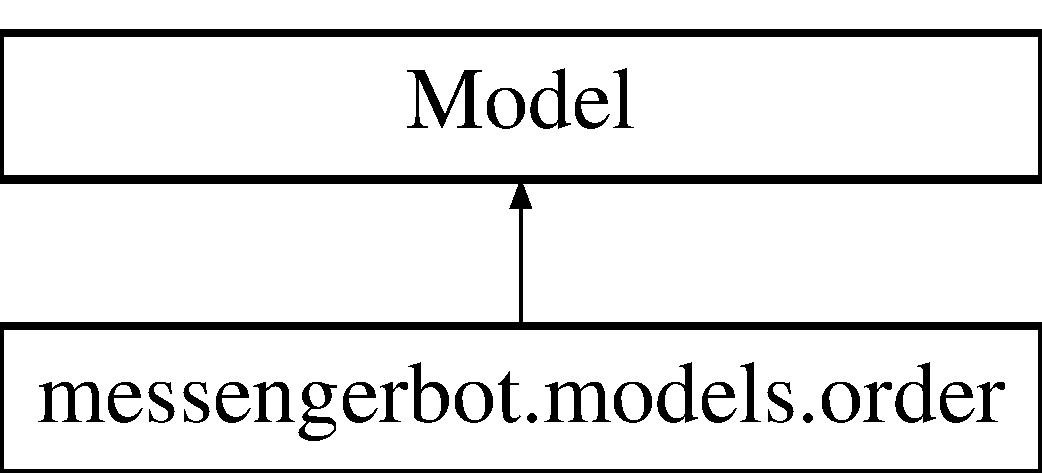
\includegraphics[height=2.000000cm]{classmessengerbot_1_1models_1_1order}
\end{center}
\end{figure}
\subsection*{Public Member Functions}
\begin{DoxyCompactItemize}
\item 
\mbox{\Hypertarget{classmessengerbot_1_1models_1_1order_a5694f24c857261d7c13d4d9e44587bab}\label{classmessengerbot_1_1models_1_1order_a5694f24c857261d7c13d4d9e44587bab}} 
def {\bfseries \+\_\+\+\_\+str\+\_\+\+\_\+} (self)
\end{DoxyCompactItemize}
\subsection*{Static Public Attributes}
\begin{DoxyCompactItemize}
\item 
\mbox{\Hypertarget{classmessengerbot_1_1models_1_1order_a6369ecae66b0caf8c6c893978bb06e58}\label{classmessengerbot_1_1models_1_1order_a6369ecae66b0caf8c6c893978bb06e58}} 
{\bfseries date} = models.\+Char\+Field(max\+\_\+length = 250 , default = \textquotesingle{}N\+U\+LL\textquotesingle{})
\item 
\mbox{\Hypertarget{classmessengerbot_1_1models_1_1order_a50cbfb1f416a825611c6bde4dc47543b}\label{classmessengerbot_1_1models_1_1order_a50cbfb1f416a825611c6bde4dc47543b}} 
{\bfseries signature\+\_\+on\+\_\+delivery} = models.\+Char\+Field(max\+\_\+length = 250 , default = \textquotesingle{}N\+U\+LL\textquotesingle{})
\item 
\mbox{\Hypertarget{classmessengerbot_1_1models_1_1order_aa09a1fd9326424c92ad881654d92f4db}\label{classmessengerbot_1_1models_1_1order_aa09a1fd9326424c92ad881654d92f4db}} 
{\bfseries description} = models.\+Char\+Field(max\+\_\+length = 250 , default = \textquotesingle{}N\+U\+LL\textquotesingle{})
\item 
\mbox{\Hypertarget{classmessengerbot_1_1models_1_1order_a503f520fd284bace2b540ea53f76d22d}\label{classmessengerbot_1_1models_1_1order_a503f520fd284bace2b540ea53f76d22d}} 
{\bfseries order\+\_\+id} = models.\+Char\+Field(max\+\_\+length = 250 , default = \textquotesingle{}N\+U\+LL\textquotesingle{})
\item 
\mbox{\Hypertarget{classmessengerbot_1_1models_1_1order_ab33a4244c1ba3ae3a22b9d631d7e9815}\label{classmessengerbot_1_1models_1_1order_ab33a4244c1ba3ae3a22b9d631d7e9815}} 
{\bfseries fbid} = models.\+Char\+Field(max\+\_\+length = 250 , default = \textquotesingle{}N\+U\+LL\textquotesingle{})
\item 
\mbox{\Hypertarget{classmessengerbot_1_1models_1_1order_a6e4c2508367c145a4e2aa8b4ac1dec9a}\label{classmessengerbot_1_1models_1_1order_a6e4c2508367c145a4e2aa8b4ac1dec9a}} 
{\bfseries type\+\_\+of\+\_\+service} = models.\+Char\+Field(max\+\_\+length = 250 , default = \textquotesingle{}N\+U\+LL\textquotesingle{})
\item 
\mbox{\Hypertarget{classmessengerbot_1_1models_1_1order_ac6a596a6158f05339945f54ae83b02a0}\label{classmessengerbot_1_1models_1_1order_ac6a596a6158f05339945f54ae83b02a0}} 
{\bfseries status} = models.\+Char\+Field(max\+\_\+length = 250 , default = \textquotesingle{}N\+U\+LL\textquotesingle{})
\item 
\mbox{\Hypertarget{classmessengerbot_1_1models_1_1order_a542b5b25ad9f273f894497e80478aabb}\label{classmessengerbot_1_1models_1_1order_a542b5b25ad9f273f894497e80478aabb}} 
{\bfseries address\+\_\+from} = models.\+Char\+Field(max\+\_\+length = 250 , default = \textquotesingle{}N\+U\+LL\textquotesingle{})
\item 
\mbox{\Hypertarget{classmessengerbot_1_1models_1_1order_a1d2d8e7fe76723170227305bc1ba79c4}\label{classmessengerbot_1_1models_1_1order_a1d2d8e7fe76723170227305bc1ba79c4}} 
{\bfseries address\+\_\+to} = models.\+Char\+Field(max\+\_\+length = 250 , default = \textquotesingle{}N\+U\+LL\textquotesingle{})
\item 
\mbox{\Hypertarget{classmessengerbot_1_1models_1_1order_a6bd62a1f2ab59c8af74c1c8c088f5928}\label{classmessengerbot_1_1models_1_1order_a6bd62a1f2ab59c8af74c1c8c088f5928}} 
{\bfseries type\+\_\+of\+\_\+shipment} = models.\+Char\+Field(max\+\_\+length = 250 , default = \textquotesingle{}N\+U\+LL\textquotesingle{})
\item 
\mbox{\Hypertarget{classmessengerbot_1_1models_1_1order_a3f34d7a4ded6a7385f05026188db3cc1}\label{classmessengerbot_1_1models_1_1order_a3f34d7a4ded6a7385f05026188db3cc1}} 
{\bfseries mode\+\_\+of\+\_\+contact} = models.\+Char\+Field(max\+\_\+length = 250 , default = \textquotesingle{}N\+U\+LL\textquotesingle{})
\item 
\mbox{\Hypertarget{classmessengerbot_1_1models_1_1order_a0c4f500101d95c3ffd496d395ab424ed}\label{classmessengerbot_1_1models_1_1order_a0c4f500101d95c3ffd496d395ab424ed}} 
{\bfseries type\+\_\+of\+\_\+collection} = models.\+Char\+Field(max\+\_\+length = 250 , default = \textquotesingle{}N\+U\+LL\textquotesingle{})
\item 
\mbox{\Hypertarget{classmessengerbot_1_1models_1_1order_a55da26eb9a52d6c13a48d27cd93a42ca}\label{classmessengerbot_1_1models_1_1order_a55da26eb9a52d6c13a48d27cd93a42ca}} 
{\bfseries type\+\_\+of\+\_\+box} = models.\+Char\+Field(max\+\_\+length = 250 , default = \textquotesingle{}N\+U\+LL\textquotesingle{})
\item 
\mbox{\Hypertarget{classmessengerbot_1_1models_1_1order_a5567b200572ec342a76f30210f08628a}\label{classmessengerbot_1_1models_1_1order_a5567b200572ec342a76f30210f08628a}} 
{\bfseries price} = models.\+Char\+Field(max\+\_\+length = 250 , default = \textquotesingle{}N\+U\+LL\textquotesingle{})
\item 
\mbox{\Hypertarget{classmessengerbot_1_1models_1_1order_ac3f038c29357b02865d2d6cd02994c8a}\label{classmessengerbot_1_1models_1_1order_ac3f038c29357b02865d2d6cd02994c8a}} 
{\bfseries picture\+\_\+state} = models.\+Integer\+Field(max\+\_\+length = 250 , default = 1)
\item 
\mbox{\Hypertarget{classmessengerbot_1_1models_1_1order_acc10f001e574003ae4617a3cd00d2e9f}\label{classmessengerbot_1_1models_1_1order_acc10f001e574003ae4617a3cd00d2e9f}} 
{\bfseries picture\+\_\+1} = models.\+Char\+Field(max\+\_\+length = 250 , default = \textquotesingle{}N\+U\+LL\textquotesingle{})
\item 
\mbox{\Hypertarget{classmessengerbot_1_1models_1_1order_a385906e5e952802d4faa7eb82edbd0dd}\label{classmessengerbot_1_1models_1_1order_a385906e5e952802d4faa7eb82edbd0dd}} 
{\bfseries picture\+\_\+2} = models.\+Char\+Field(max\+\_\+length = 250 , default = \textquotesingle{}N\+U\+LL\textquotesingle{})
\end{DoxyCompactItemize}


The documentation for this class was generated from the following file\+:\begin{DoxyCompactItemize}
\item 
models.\+py\end{DoxyCompactItemize}

\hypertarget{classmessengerbot_1_1models_1_1place}{}\section{messengerbot.\+models.\+place Class Reference}
\label{classmessengerbot_1_1models_1_1place}\index{messengerbot.\+models.\+place@{messengerbot.\+models.\+place}}
Inheritance diagram for messengerbot.\+models.\+place\+:\begin{figure}[H]
\begin{center}
\leavevmode
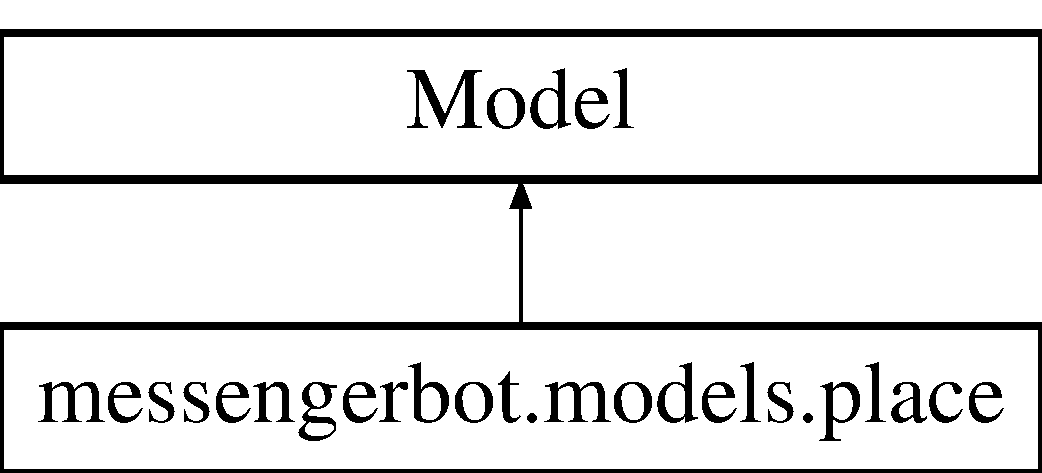
\includegraphics[height=2.000000cm]{classmessengerbot_1_1models_1_1place}
\end{center}
\end{figure}
\subsection*{Public Member Functions}
\begin{DoxyCompactItemize}
\item 
\mbox{\Hypertarget{classmessengerbot_1_1models_1_1place_ac181d9c7d3b1926c65008ba8b28efba5}\label{classmessengerbot_1_1models_1_1place_ac181d9c7d3b1926c65008ba8b28efba5}} 
def {\bfseries \+\_\+\+\_\+str\+\_\+\+\_\+} (self)
\end{DoxyCompactItemize}
\subsection*{Static Public Attributes}
\begin{DoxyCompactItemize}
\item 
\mbox{\Hypertarget{classmessengerbot_1_1models_1_1place_ae0d24c4671e9ce38726f84ce8ceb0103}\label{classmessengerbot_1_1models_1_1place_ae0d24c4671e9ce38726f84ce8ceb0103}} 
{\bfseries name} = models.\+Char\+Field(max\+\_\+length = 250 , default = \textquotesingle{}N\+U\+LL\textquotesingle{})
\item 
\mbox{\Hypertarget{classmessengerbot_1_1models_1_1place_afba837819d7d201fd5862ec7af55825f}\label{classmessengerbot_1_1models_1_1place_afba837819d7d201fd5862ec7af55825f}} 
{\bfseries timezone} = models.\+Char\+Field(max\+\_\+length = 250 , default = \textquotesingle{}N\+U\+LL\textquotesingle{})
\item 
\mbox{\Hypertarget{classmessengerbot_1_1models_1_1place_a1446d5fdbadcd68a658aab909504dc21}\label{classmessengerbot_1_1models_1_1place_a1446d5fdbadcd68a658aab909504dc21}} 
{\bfseries country} = models.\+Foreign\+Key(\hyperlink{classmessengerbot_1_1models_1_1country}{country}, on\+\_\+delete=models.\+C\+A\+S\+C\+A\+DE)
\item 
\mbox{\Hypertarget{classmessengerbot_1_1models_1_1place_a84e97bec05192c2bbdd3123732896d2e}\label{classmessengerbot_1_1models_1_1place_a84e97bec05192c2bbdd3123732896d2e}} 
{\bfseries languages} = models.\+Many\+To\+Many\+Field(\hyperlink{classmessengerbot_1_1models_1_1language}{language}, null = True)
\end{DoxyCompactItemize}


\subsection{Detailed Description}
\begin{DoxyVerb}places DHL work in \end{DoxyVerb}
 

The documentation for this class was generated from the following file\+:\begin{DoxyCompactItemize}
\item 
models.\+py\end{DoxyCompactItemize}

\hypertarget{classmessengerbot_1_1models_1_1status}{}\section{messengerbot.\+models.\+status Class Reference}
\label{classmessengerbot_1_1models_1_1status}\index{messengerbot.\+models.\+status@{messengerbot.\+models.\+status}}
Inheritance diagram for messengerbot.\+models.\+status\+:\begin{figure}[H]
\begin{center}
\leavevmode
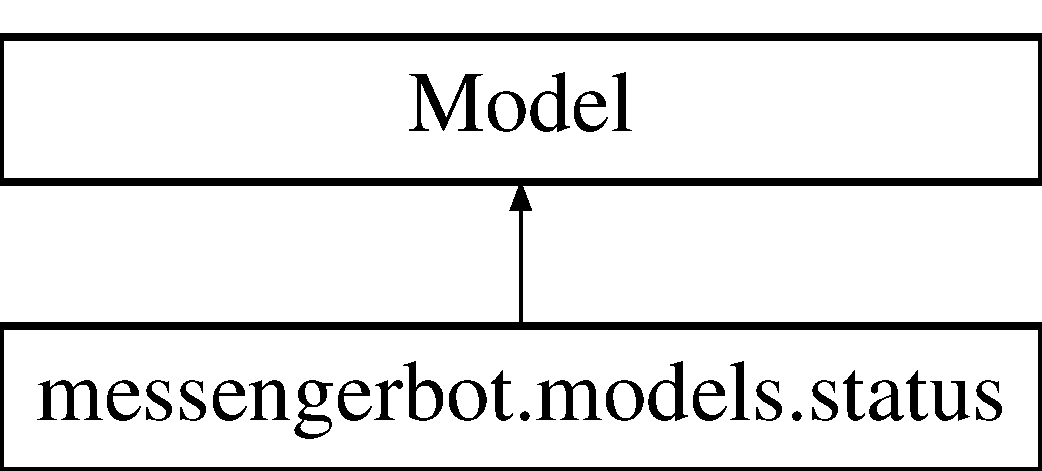
\includegraphics[height=2.000000cm]{classmessengerbot_1_1models_1_1status}
\end{center}
\end{figure}
\subsection*{Public Member Functions}
\begin{DoxyCompactItemize}
\item 
\mbox{\Hypertarget{classmessengerbot_1_1models_1_1status_a8118d8d2338a4499e11a1edca485732b}\label{classmessengerbot_1_1models_1_1status_a8118d8d2338a4499e11a1edca485732b}} 
def {\bfseries \+\_\+\+\_\+str\+\_\+\+\_\+} (self)
\end{DoxyCompactItemize}
\subsection*{Static Public Attributes}
\begin{DoxyCompactItemize}
\item 
\mbox{\Hypertarget{classmessengerbot_1_1models_1_1status_a0a3e686172dda050ed397e3c02dd0e90}\label{classmessengerbot_1_1models_1_1status_a0a3e686172dda050ed397e3c02dd0e90}} 
{\bfseries status} = models.\+Foreign\+Key(\hyperlink{classmessengerbot_1_1models_1_1status__code}{status\+\_\+code} , related\+\_\+name=\textquotesingle{}status\+Message\textquotesingle{}, on\+\_\+delete=models.\+C\+A\+S\+C\+A\+DE)
\item 
\mbox{\Hypertarget{classmessengerbot_1_1models_1_1status_a63f065ddf8a8fc756041f554c70d90ba}\label{classmessengerbot_1_1models_1_1status_a63f065ddf8a8fc756041f554c70d90ba}} 
{\bfseries timestamp} = models.\+Date\+Time\+Field(blank = True , null = True)
\item 
\mbox{\Hypertarget{classmessengerbot_1_1models_1_1status_af9593cfd65b337505e2702a35ada7839}\label{classmessengerbot_1_1models_1_1status_af9593cfd65b337505e2702a35ada7839}} 
{\bfseries location} = models.\+Char\+Field(max\+\_\+length = 250 , default = \textquotesingle{}N\+U\+LL\textquotesingle{})
\end{DoxyCompactItemize}


The documentation for this class was generated from the following file\+:\begin{DoxyCompactItemize}
\item 
models.\+py\end{DoxyCompactItemize}

\hypertarget{classmessengerbot_1_1models_1_1status__code}{}\section{messengerbot.\+models.\+status\+\_\+code Class Reference}
\label{classmessengerbot_1_1models_1_1status__code}\index{messengerbot.\+models.\+status\+\_\+code@{messengerbot.\+models.\+status\+\_\+code}}
Inheritance diagram for messengerbot.\+models.\+status\+\_\+code\+:\begin{figure}[H]
\begin{center}
\leavevmode
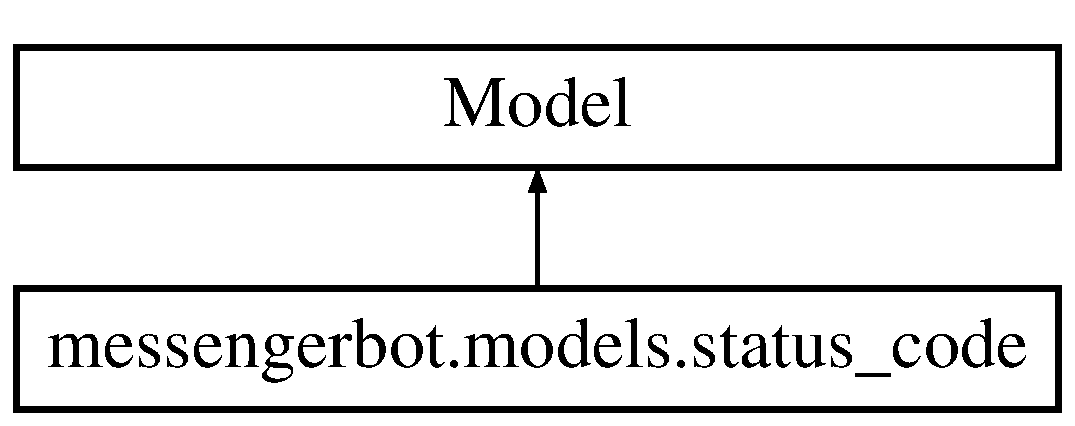
\includegraphics[height=2.000000cm]{classmessengerbot_1_1models_1_1status__code}
\end{center}
\end{figure}
\subsection*{Public Member Functions}
\begin{DoxyCompactItemize}
\item 
\mbox{\Hypertarget{classmessengerbot_1_1models_1_1status__code_a26cab58d40b51e434242f6a324e0247c}\label{classmessengerbot_1_1models_1_1status__code_a26cab58d40b51e434242f6a324e0247c}} 
def {\bfseries \+\_\+\+\_\+str\+\_\+\+\_\+} (self)
\end{DoxyCompactItemize}
\subsection*{Static Public Attributes}
\begin{DoxyCompactItemize}
\item 
\mbox{\Hypertarget{classmessengerbot_1_1models_1_1status__code_a61285a10b7a60b3a8f87504194bea9f5}\label{classmessengerbot_1_1models_1_1status__code_a61285a10b7a60b3a8f87504194bea9f5}} 
{\bfseries status} = models.\+Char\+Field(max\+\_\+length = 250 , default = \textquotesingle{}N\+U\+LL\textquotesingle{})
\end{DoxyCompactItemize}


\subsection{Detailed Description}
\begin{DoxyVerb}for all the status messages provided by dhl for eg: The instruction data for this shipment have been provided by the sender to DHL electronically\end{DoxyVerb}
 

The documentation for this class was generated from the following file\+:\begin{DoxyCompactItemize}
\item 
models.\+py\end{DoxyCompactItemize}

\hypertarget{classmessengerbot_1_1tests_1_1TestVerifyToken}{}\section{messengerbot.\+tests.\+Test\+Verify\+Token Class Reference}
\label{classmessengerbot_1_1tests_1_1TestVerifyToken}\index{messengerbot.\+tests.\+Test\+Verify\+Token@{messengerbot.\+tests.\+Test\+Verify\+Token}}
Inheritance diagram for messengerbot.\+tests.\+Test\+Verify\+Token\+:\begin{figure}[H]
\begin{center}
\leavevmode
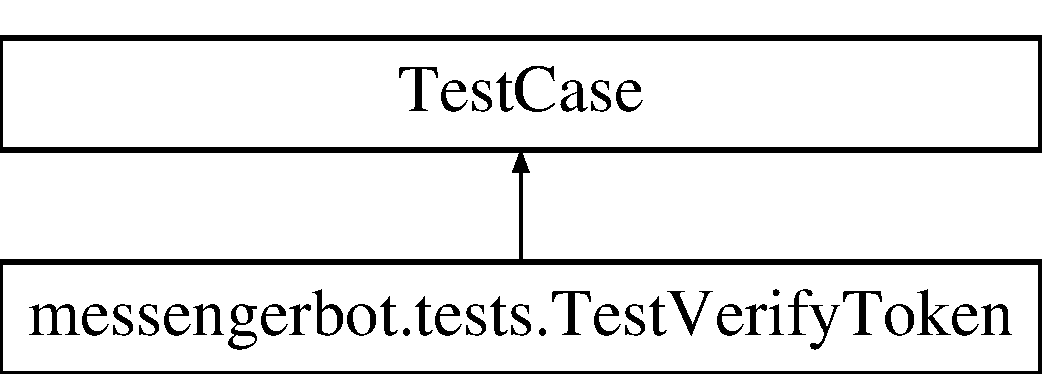
\includegraphics[height=2.000000cm]{classmessengerbot_1_1tests_1_1TestVerifyToken}
\end{center}
\end{figure}
\subsection*{Public Member Functions}
\begin{DoxyCompactItemize}
\item 
\mbox{\Hypertarget{classmessengerbot_1_1tests_1_1TestVerifyToken_a1613e92792aa6bd97d7056b5d68dee6a}\label{classmessengerbot_1_1tests_1_1TestVerifyToken_a1613e92792aa6bd97d7056b5d68dee6a}} 
def \hyperlink{classmessengerbot_1_1tests_1_1TestVerifyToken_a1613e92792aa6bd97d7056b5d68dee6a}{test\+\_\+\+Verify\+Token} (self)
\begin{DoxyCompactList}\small\item\em testing for the correct response \end{DoxyCompactList}\end{DoxyCompactItemize}


The documentation for this class was generated from the following file\+:\begin{DoxyCompactItemize}
\item 
tests.\+py\end{DoxyCompactItemize}

\hypertarget{classmessengerbot_1_1models_1_1type__of__box}{}\section{messengerbot.\+models.\+type\+\_\+of\+\_\+box Class Reference}
\label{classmessengerbot_1_1models_1_1type__of__box}\index{messengerbot.\+models.\+type\+\_\+of\+\_\+box@{messengerbot.\+models.\+type\+\_\+of\+\_\+box}}
Inheritance diagram for messengerbot.\+models.\+type\+\_\+of\+\_\+box\+:\begin{figure}[H]
\begin{center}
\leavevmode
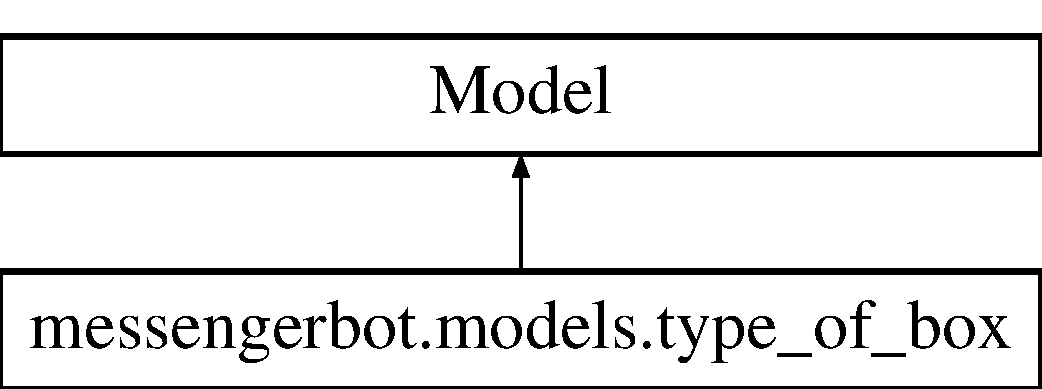
\includegraphics[height=2.000000cm]{classmessengerbot_1_1models_1_1type__of__box}
\end{center}
\end{figure}
\subsection*{Public Member Functions}
\begin{DoxyCompactItemize}
\item 
\mbox{\Hypertarget{classmessengerbot_1_1models_1_1type__of__box_ab6bfc5fff4cd1d8144d037d559cbb932}\label{classmessengerbot_1_1models_1_1type__of__box_ab6bfc5fff4cd1d8144d037d559cbb932}} 
def {\bfseries \+\_\+\+\_\+str\+\_\+\+\_\+} (self)
\end{DoxyCompactItemize}
\subsection*{Static Public Attributes}
\begin{DoxyCompactItemize}
\item 
\mbox{\Hypertarget{classmessengerbot_1_1models_1_1type__of__box_a42410a03c6abf8fe27bb9b21ba3abe42}\label{classmessengerbot_1_1models_1_1type__of__box_a42410a03c6abf8fe27bb9b21ba3abe42}} 
{\bfseries type\+\_\+of\+\_\+box} = models.\+Char\+Field(max\+\_\+length = 250 , default = \textquotesingle{}N\+U\+LL\textquotesingle{})
\end{DoxyCompactItemize}


\subsection{Detailed Description}
\begin{DoxyVerb}for type of containers like envolope , box 1 , box 2 , box 3 etc.\end{DoxyVerb}
 

The documentation for this class was generated from the following file\+:\begin{DoxyCompactItemize}
\item 
models.\+py\end{DoxyCompactItemize}

\hypertarget{classmessengerbot_1_1models_1_1type__of__collection}{}\section{messengerbot.\+models.\+type\+\_\+of\+\_\+collection Class Reference}
\label{classmessengerbot_1_1models_1_1type__of__collection}\index{messengerbot.\+models.\+type\+\_\+of\+\_\+collection@{messengerbot.\+models.\+type\+\_\+of\+\_\+collection}}
Inheritance diagram for messengerbot.\+models.\+type\+\_\+of\+\_\+collection\+:\begin{figure}[H]
\begin{center}
\leavevmode
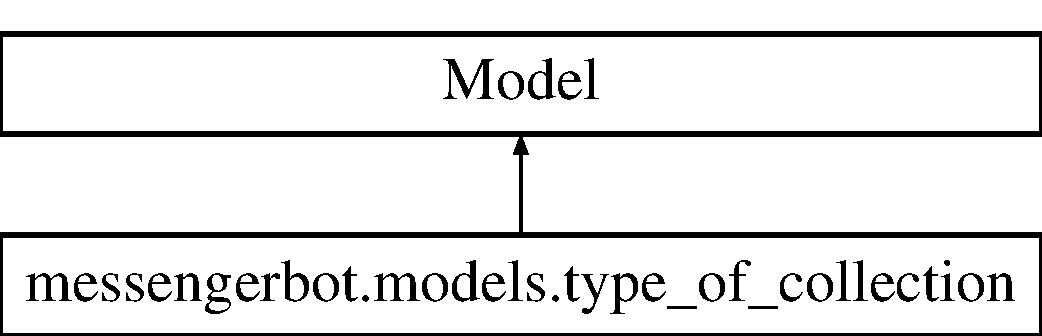
\includegraphics[height=2.000000cm]{classmessengerbot_1_1models_1_1type__of__collection}
\end{center}
\end{figure}
\subsection*{Public Member Functions}
\begin{DoxyCompactItemize}
\item 
\mbox{\Hypertarget{classmessengerbot_1_1models_1_1type__of__collection_a1b6a6ac597b4c84bfd6a96bfaedfc708}\label{classmessengerbot_1_1models_1_1type__of__collection_a1b6a6ac597b4c84bfd6a96bfaedfc708}} 
def {\bfseries \+\_\+\+\_\+str\+\_\+\+\_\+} (self)
\end{DoxyCompactItemize}
\subsection*{Static Public Attributes}
\begin{DoxyCompactItemize}
\item 
\mbox{\Hypertarget{classmessengerbot_1_1models_1_1type__of__collection_a2d65815b76f23bad35232b6c926aed23}\label{classmessengerbot_1_1models_1_1type__of__collection_a2d65815b76f23bad35232b6c926aed23}} 
{\bfseries type\+\_\+of\+\_\+collection} = models.\+Char\+Field(max\+\_\+length = 250 , default = \textquotesingle{}N\+U\+LL\textquotesingle{})
\end{DoxyCompactItemize}


The documentation for this class was generated from the following file\+:\begin{DoxyCompactItemize}
\item 
models.\+py\end{DoxyCompactItemize}

\hypertarget{classmessengerbot_1_1models_1_1type__of__service}{}\section{messengerbot.\+models.\+type\+\_\+of\+\_\+service Class Reference}
\label{classmessengerbot_1_1models_1_1type__of__service}\index{messengerbot.\+models.\+type\+\_\+of\+\_\+service@{messengerbot.\+models.\+type\+\_\+of\+\_\+service}}
Inheritance diagram for messengerbot.\+models.\+type\+\_\+of\+\_\+service\+:\begin{figure}[H]
\begin{center}
\leavevmode
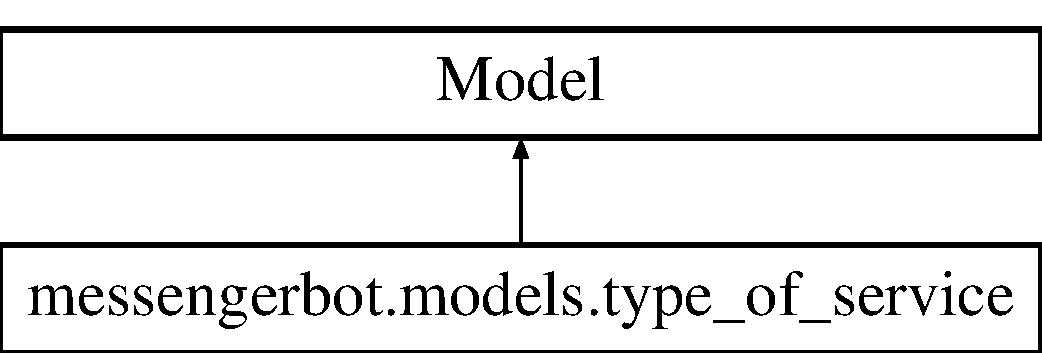
\includegraphics[height=2.000000cm]{classmessengerbot_1_1models_1_1type__of__service}
\end{center}
\end{figure}
\subsection*{Public Member Functions}
\begin{DoxyCompactItemize}
\item 
\mbox{\Hypertarget{classmessengerbot_1_1models_1_1type__of__service_ab573c9cf8659e781a2c3ddd8741ff7d2}\label{classmessengerbot_1_1models_1_1type__of__service_ab573c9cf8659e781a2c3ddd8741ff7d2}} 
def {\bfseries \+\_\+\+\_\+str\+\_\+\+\_\+} (self)
\end{DoxyCompactItemize}
\subsection*{Static Public Attributes}
\begin{DoxyCompactItemize}
\item 
\mbox{\Hypertarget{classmessengerbot_1_1models_1_1type__of__service_a00cc860399c8c70331308d118f5677c9}\label{classmessengerbot_1_1models_1_1type__of__service_a00cc860399c8c70331308d118f5677c9}} 
{\bfseries type\+\_\+of\+\_\+service} = models.\+Char\+Field(max\+\_\+length = 250 , default = \textquotesingle{}N\+U\+LL\textquotesingle{})
\end{DoxyCompactItemize}


The documentation for this class was generated from the following file\+:\begin{DoxyCompactItemize}
\item 
models.\+py\end{DoxyCompactItemize}

\hypertarget{classmessengerbot_1_1models_1_1type__of__shipment}{}\section{messengerbot.\+models.\+type\+\_\+of\+\_\+shipment Class Reference}
\label{classmessengerbot_1_1models_1_1type__of__shipment}\index{messengerbot.\+models.\+type\+\_\+of\+\_\+shipment@{messengerbot.\+models.\+type\+\_\+of\+\_\+shipment}}
Inheritance diagram for messengerbot.\+models.\+type\+\_\+of\+\_\+shipment\+:\begin{figure}[H]
\begin{center}
\leavevmode
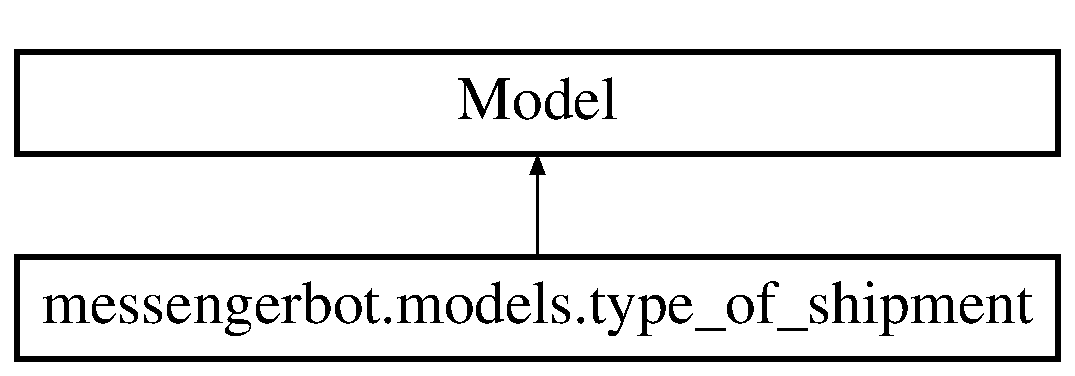
\includegraphics[height=2.000000cm]{classmessengerbot_1_1models_1_1type__of__shipment}
\end{center}
\end{figure}
\subsection*{Public Member Functions}
\begin{DoxyCompactItemize}
\item 
\mbox{\Hypertarget{classmessengerbot_1_1models_1_1type__of__shipment_ad991877bb87d7bca5e8c0bae090c145e}\label{classmessengerbot_1_1models_1_1type__of__shipment_ad991877bb87d7bca5e8c0bae090c145e}} 
def {\bfseries \+\_\+\+\_\+str\+\_\+\+\_\+} (self)
\end{DoxyCompactItemize}
\subsection*{Static Public Attributes}
\begin{DoxyCompactItemize}
\item 
\mbox{\Hypertarget{classmessengerbot_1_1models_1_1type__of__shipment_a679547579bf080f1baee36b9f974ca3f}\label{classmessengerbot_1_1models_1_1type__of__shipment_a679547579bf080f1baee36b9f974ca3f}} 
{\bfseries type\+\_\+of\+\_\+shipment} = models.\+Char\+Field(max\+\_\+length = 250 , default = \textquotesingle{}N\+U\+LL\textquotesingle{})
\end{DoxyCompactItemize}


The documentation for this class was generated from the following file\+:\begin{DoxyCompactItemize}
\item 
models.\+py\end{DoxyCompactItemize}

\hypertarget{classmessengerbot_1_1models_1_1user}{}\section{messengerbot.\+models.\+user Class Reference}
\label{classmessengerbot_1_1models_1_1user}\index{messengerbot.\+models.\+user@{messengerbot.\+models.\+user}}
Inheritance diagram for messengerbot.\+models.\+user\+:\begin{figure}[H]
\begin{center}
\leavevmode
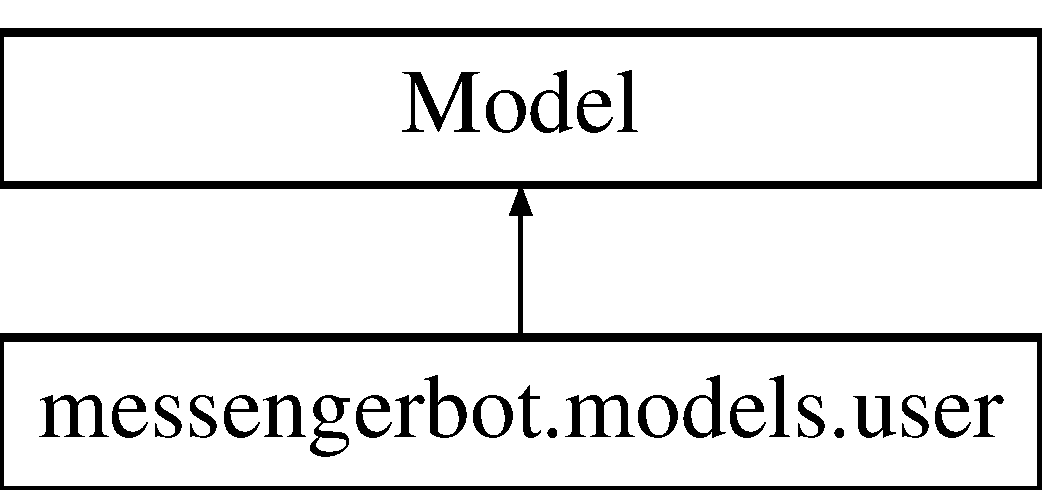
\includegraphics[height=2.000000cm]{classmessengerbot_1_1models_1_1user}
\end{center}
\end{figure}
\subsection*{Public Member Functions}
\begin{DoxyCompactItemize}
\item 
\mbox{\Hypertarget{classmessengerbot_1_1models_1_1user_a3f5e43e7673443ae3715bcb51416a735}\label{classmessengerbot_1_1models_1_1user_a3f5e43e7673443ae3715bcb51416a735}} 
def {\bfseries \+\_\+\+\_\+str\+\_\+\+\_\+} (self)
\end{DoxyCompactItemize}
\subsection*{Static Public Attributes}
\begin{DoxyCompactItemize}
\item 
\mbox{\Hypertarget{classmessengerbot_1_1models_1_1user_a006ce81d6b1219a617fb3a0d1b5c06d1}\label{classmessengerbot_1_1models_1_1user_a006ce81d6b1219a617fb3a0d1b5c06d1}} 
{\bfseries mobile} = models.\+Char\+Field(max\+\_\+length = 250 , default = \textquotesingle{}N\+U\+LL\textquotesingle{})
\item 
\mbox{\Hypertarget{classmessengerbot_1_1models_1_1user_a465b6800ae148440932d8984f6770637}\label{classmessengerbot_1_1models_1_1user_a465b6800ae148440932d8984f6770637}} 
{\bfseries fbid} = models.\+Char\+Field(max\+\_\+length = 250 , default = \textquotesingle{}N\+U\+LL\textquotesingle{})
\item 
\mbox{\Hypertarget{classmessengerbot_1_1models_1_1user_ad88b250ebdac82d889b30f31d6339754}\label{classmessengerbot_1_1models_1_1user_ad88b250ebdac82d889b30f31d6339754}} 
{\bfseries name} = models.\+Char\+Field(max\+\_\+length = 250 , default = \textquotesingle{}N\+U\+LL\textquotesingle{})
\item 
\mbox{\Hypertarget{classmessengerbot_1_1models_1_1user_a13e9e7fd31136cc8713e0d0f98c6c9aa}\label{classmessengerbot_1_1models_1_1user_a13e9e7fd31136cc8713e0d0f98c6c9aa}} 
{\bfseries email} = models.\+Char\+Field(max\+\_\+length = 250 , default = \textquotesingle{}N\+U\+LL\textquotesingle{})
\end{DoxyCompactItemize}


\subsection{Detailed Description}
\begin{DoxyVerb}user data of the people interacting with the bot \end{DoxyVerb}
 

The documentation for this class was generated from the following file\+:\begin{DoxyCompactItemize}
\item 
models.\+py\end{DoxyCompactItemize}

%--- End generated contents ---

% Index
\backmatter
\newpage
\phantomsection
\clearemptydoublepage
\addcontentsline{toc}{chapter}{Index}
\printindex

\end{document}
